\documentclass[titlepage]{article}

\usepackage{setspace}

\usepackage[utf8]{inputenc}
\usepackage{amsmath}   
\usepackage{mathtools}
\usepackage{graphicx}
\usepackage{subcaption}
\usepackage{float}
\usepackage{hyperref}
\usepackage{listings}
\usepackage[labelfont=bf]{caption}
\usepackage[margin=3.5cm]{geometry}

%\usepackage{qtree}
%\usepackage{tikz}
%\usepackage{tikz-qtree}

%\usepackage[]{algorithm2e}

\lstset{
	basicstyle=\footnotesize\ttfamily,
}

\title{
\vspace{80pt}\\
\LARGE \bfseries SKEDGE
\\\vspace{10pt}\Large Smarter course scheduling for our\\University of Rochester
}

\author{
	Dan Hassin\\
    \vspace{5pt}\\
    Supervised by Professor Philip Guo\\
    \vspace{5pt}\\
    Department of Computer Science\\
    University of Rochester\\
    Rochester, New York\\
}

\date{April 12, 2016\\
    \vspace{150pt}\\
    submitted in partial fulfillment of\\
    the requirements for the degree\\
    honors bachelor of science\\
}

\begin{document}

\maketitle

\doublespacing

% Direct search for specific course
% Discovery, browsing, exploring
% behavioral patterns

% STAT: Find major of users, find how many non-major courses they found

\begin{abstract}

In this paper I present Skedge, a web application for students to comfortably and effectively engage with the University's course catalog. Skedge matches and surpasses the capabilities of the existing University tool for this purpose, ``Course Description / Course Schedule'' (CDCS) and presents its information in a more visually pleasing way. As a result, Skedge boasts strong user-retention rates, long session durations, and high student adoption despite having virtually no advertisement. Through collected usage data, I demonstrate that a) Skedge's differences from and additions to CDCS are usable and have real need, b) the two major use-cases associated with course browsing---direct search and exploratory search---are effectively accommodated by Skedge, and c) Skedge's search mechanism is user-friendly and self-teaches to users over time.

\end{abstract}

\begin{figure}[ht]
    \centering
    \begin{tabular}{c c}
        \begin{subfigure}[h]{6.5cm}
            \centering
            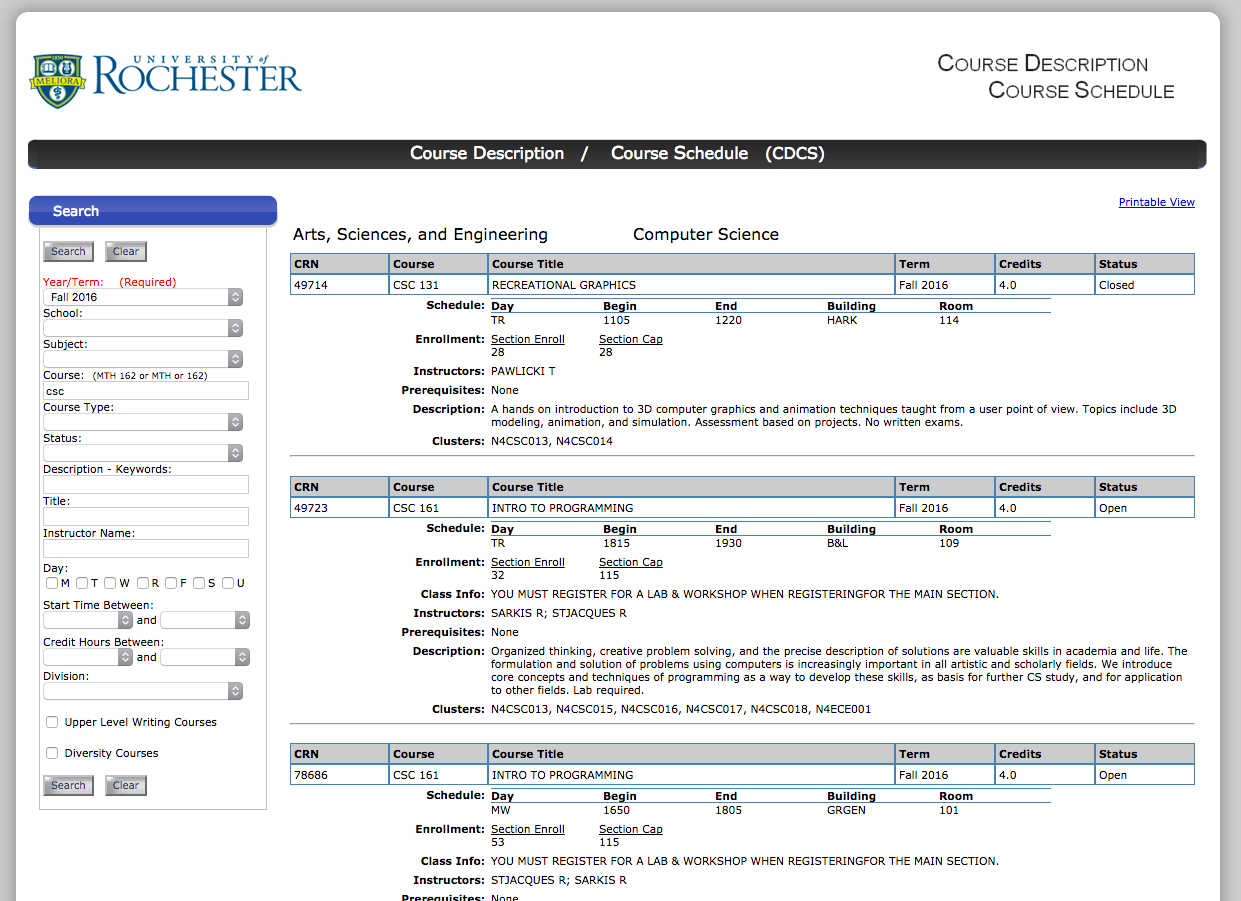
\includegraphics[width=1.00\textwidth]{images/cdcs}
        \end{subfigure}
        \hspace{1em}
        \begin{subfigure}[h]{7.5cm}
            \centering
            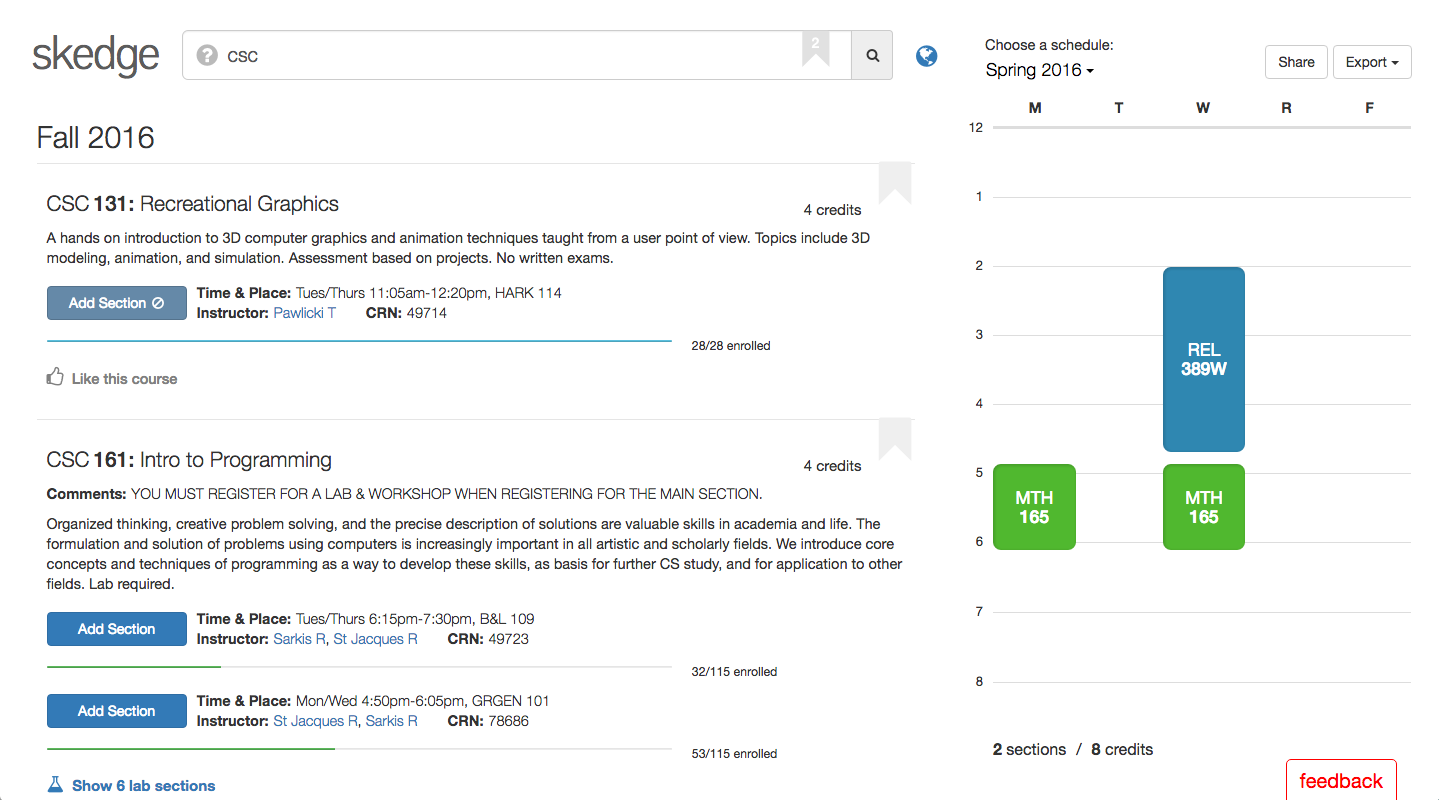
\includegraphics[width=1.00\textwidth]{images/skedge}
        \end{subfigure}
    \end{tabular}
    \caption{CDCS (left) and Skedge (right) for the search query {\tt csc}.}
\end{figure}

\section{Introduction}

This paper\cite{escodegen} will begin by discussing Markov chains and how we set out to use them for our goal of creating an assistive program editor. We will then describe in detail how we implemented a Markov chain to house program syntax trees, how we were able to generate code using it, and finally we'll discuss our results and address the limitations of our product.

\subsection{Markov chain}

A Markov chain is a mathematical system that undergoes a stochastic process whereby


\subsection*{Source code \& live site}

The source code for Skedge is available online under an open
source license:
\url{https://github.com/RocHack/skedge}.\\

\noindent The site can be found at
\url{http://skedgeur.com}.

\clearpage

\begin{thebibliography}{1}

	\bibitem{esprima} Ariya Hidayat {\em Esprima}
		\\\url{http://esprima.org/}

	\bibitem{markov} Takis Konstantopoulos {\em Introductory lecture notes on
		Markov Chains and Random Walks.} Uppsala University,
		\\\url{http://www2.math.uu.se/~takis/L/McRw/mcrw.pdf}

	\bibitem{hosa} Frank Pfenning, Conal Elliott
		{\em Higher-Order Abstract Syntax.}
		ACM SIGPLAN Notices. Vol. 23. No. 7. ACM, 1988.
		\\\url{http://www.cs.cmu.edu/~fp/papers/pldi88.pdf}

	\bibitem{escodegen} Yusuke Suzuki {\em Escodegen}
		\\\url{https://github.com/Constellation/escodegen}

	\bibitem{parser api} Mozilla Developer Network {\em SpiderMonkey Parser API}
		\\\url{https://developer.mozilla.org/en-US/docs/SpiderMonkey/Parser_API}

\end{thebibliography}

\clearpage
\section*{Appendix}

\end{document}
